
\subsection{Background}
Consider the strictly convex\footnote{The case when $Q \succeq 0$ is treated in a later section.} quadratic program
\begin{equation}\label{eq:qp}
\begin{aligned}
\min_{x \in \mathbb{R}^n} \quad & f(x) = \tfrac{1}{2}x^\top Q x + g^\top x \\
\text{subject to} \quad & a_i^\top x \leq b_i, \quad i = 1,\ldots,m,
\end{aligned}
\end{equation}
where $Q\succ0$ and the feasible region
\[
\mathcal P = \{x\in\mathbb R^n : Ax\le b\}
\]
is a polytope.

\noindent In this work we focus on the class of problems in which $\mathcal{P}$ is a box or, more generally, an affine image of a box. That is, $\mathcal{P}$ can be written as
\[
\mathcal{P} = T(\mathcal{B}) = \{Tx + c : x \in \mathcal{B}\},
\]
where $T \in \mathbb{R}^{n\times n}$ is nonsingular, $c \in \mathbb{R}^n$, and
\[
\mathcal{B} = \{x \in \mathbb{R}^n : \ell \le x \le u\}
\]
is an axis-aligned box defined by lower and upper bounds $\ell,u \in \mathbb{R}^n$ with $\ell < u$ componentwise.
\begin{remark}\label{rem:halfspace-rep-boxes}
The half-space representation of $\mathcal P$ can be written as
\[
A =
\begin{bmatrix}
T^{-1} \\ -T^{-1}
\end{bmatrix},
\qquad
b =
\begin{bmatrix}
u + T^{-1}c \\ -\ell - T^{-1}c
\end{bmatrix}.
\]
\end{remark}

\noindent Let $\bar x=-Q^{-1}g$ denote the unconstrained minimizer.
Throughout we assume $\bar x\notin\mathcal P$.

For $\mathcal I\subseteq\{1,\dots,m\}$ define
\[
F(\mathcal I)
=
\{x\in\mathcal P : a_i^\top x=b_i,\ i\in\mathcal I\}.
\]
A nonempty set of this form is called a \emph{face} of $\mathcal P$.
Faces of dimension $n-1$, $n-2$ and $0$ are called \emph{facets}, \emph{ridges} and \emph{vertices}, respectively. Two facets are said to be \emph{adjacent} if they share a common ridge.

For a feasible point $x\in\mathcal P$ we denote the active set by
\[
\mathcal A(x)=\{i: a_i^\top x=b_i\}.
\]
A central object of this paper is the notion of a \emph{good vertex} relative to an exterior point.
\begin{definition}\label{def:good_vertex}
Let $\bar{x} \notin \mathcal{P}$. A vertex $v$ of $\mathcal{P}$ is called
\emph{good} (with respect to $\bar{x}$) if the ray from $v$ toward $\bar{x}$
initially enters the interior of $\mathcal{P}$, i.e.,
\[
v + t(\bar{x}-v) \in \relint(\mathcal P)
\quad \text{for all sufficiently small } t>0 .
\]
Equivalently,
\[
a_i^\top(\bar{x}-v) < 0
\quad \text{for all } i \in \mathcal A(v).
\]
\end{definition}

\begin{remark}
Geometrically, a vertex is good if $\bar{x}$ lies inside the cone generated
by the edges of $\mathcal P$ incident to $v$.
\end{remark}

\begin{lemma}
Let $\mathcal P = T(\mathcal B)+c,
\quad
\mathcal B = \{y\in\mathbb R^n : \ell \le y \le u\},
$ 
where $T\in\mathbb R^{n\times n}$ is nonsingular and $\ell<u$ component-wise.
Let $\bar x \notin \mathcal P$, and define $\bar y := T^{-1}(\bar x-c)$.

\begin{enumerate}
\item[(i)] The set $V_\text{good}$ of good vertices of $\mathcal P$ (with respect to $\bar x$) is nonempty.

\item[(ii)] A vertex $v\in\mathcal P$ is good if and only if $v=Ty+c$, where $y$ is a vertex of $\mathcal B$ satisfying
\[
\begin{cases}
y_i=\ell_i \ \Rightarrow\ \bar y_i>\ell_i,\\
y_i=u_i \ \Rightarrow\ \bar y_i<u_i,
\end{cases}
\qquad i=1,\dots,n.
\]
\end{enumerate}
\end{lemma}

\begin{proof}
Let $v=Ty+c$ be a vertex of $\mathcal P$, where $y$ is a vertex of $\mathcal B$.
The active constraints at $v$ correspond to
\[
\begin{cases}
(T^{-1})_{i,\cdot}(x-c) \le u_i & \text{if } y_i=u_i,\\
-(T^{-1})_{i,\cdot}(x-c) \le -\ell_i & \text{if } y_i=\ell_i.
\end{cases}
\]
Hence
\[
a_i^\top(\bar x - v)
=
\begin{cases}
\bar y_i - u_i & \text{if } y_i=u_i,\\
-(\bar y_i - \ell_i) & \text{if } y_i=\ell_i,
\end{cases}
\]
so $v$ is good if and only if
\[
\begin{cases}
\bar y_i < u_i & \text{if } y_i=u_i,\\
\bar y_i > \ell_i & \text{if } y_i=\ell_i,
\end{cases}
\]
which proves (ii). To show (i), note that $\bar x \notin \mathcal P$ implies $\bar y \notin \mathcal B$, so $\bar y_i \notin [\ell_i,u_i] \ \text{for at least one } i,
$
and in particular, for every $i$ at least one of the strict inequalities
$\bar y_i > \ell_i$ or $\bar y_i < u_i$ holds. Define $y\in\mathcal B$ component-wise by
\[
y_i :=
\begin{cases}
\ell_i & \text{if } \bar y_i > \ell_i,\\
u_i & \text{if } \bar y_i < u_i.
\end{cases}
\]
This definition is well posed (at least one case always applies), and yields a vertex $y$ of $\mathcal B$. Moreover, by construction,
\[
y_i=\ell_i \ \Rightarrow\ \bar y_i>\ell_i,
\qquad
y_i=u_i \ \Rightarrow\ \bar y_i<u_i,
\]
for all $i$. By part (ii), the vertex $v=Ty+c$ is therefore good. This proves (i).
\end{proof}

\begin{figure}[t!]
\centering
\fbox{
\begin{minipage}{0.95\textwidth}
\centering
\begin{subfigure}[b]{0.3\textwidth}
\centering
\begin{tikzpicture}[scale=1.1]
\coordinate (v1) at (1,0); \coordinate (v2) at (2,0.5);
\coordinate (v3) at (2.5,1.5); \coordinate (v4) at (2,2.5);
\coordinate (v5) at (1,3); \coordinate (v6) at (0,2.5);
\coordinate (v7) at (-0.5,1.5); \coordinate (v8) at (0,0.5);
\draw[thick] (v1) -- (v2) -- (v3) -- (v4) -- (v5) -- (v6) -- (v7) -- (v8) -- cycle;
\fill[blue!10] (v1) -- (v2) -- (v3) -- (v4) -- (v5) -- (v6) -- (v7) -- (v8) -- cycle;
\coordinate (xbar) at (3.5,1.5); \filldraw[red] (xbar) circle (2pt); \node[above right] at (xbar) {$\bar{x}$};
\foreach \v in {v6,v7,v8} {\filldraw[green!70!black] (\v) circle (2.5pt);}
\draw[dashed,->,green!70!black] (v6) -- ($(v6)!0.9!(xbar)$);
\draw[dashed,->,green!70!black] (v7) -- ($(v7)!0.9!(xbar)$);
\draw[dashed,->,green!70!black] (v8) -- ($(v8)!0.9!(xbar)$);
\end{tikzpicture}
\caption{Several good vertices}
\end{subfigure}
\hfill
\begin{subfigure}[b]{0.3\textwidth}
\centering
\begin{tikzpicture}[scale=3.5,tdplot_main_coords]
\tdplotsetmaincoords{60}{120}

\coordinate (v1) at (0,0,0); 
\coordinate (v2) at (1,0,0);
\coordinate (v3) at (0.5,0.866,0);
\coordinate (v4) at (0.5,0.289,0.816); 

\draw[thick] (v1) -- (v2) -- (v3) -- cycle;
\draw[thick] (v1) -- (v4); \draw[thick] (v2) -- (v4); \draw[thick] (v3) -- (v4);

\fill[blue!10,opacity=0.5] (v1) -- (v2) -- (v3) -- cycle;
\fill[blue!10,opacity=0.5] (v1) -- (v2) -- (v4) -- cycle;
\fill[blue!10,opacity=0.5] (v2) -- (v3) -- (v4) -- cycle;
\fill[blue!10,opacity=0.5] (v3) -- (v1) -- (v4) -- cycle;

\coordinate (xbar) at (1.4,0.5,0.8); \filldraw[red] (xbar) circle (0.8pt); \node[above] at (xbar) {$\bar{x}$};

\filldraw[green!70!black] (v1) circle (0.8pt); 
%\node[left] at (v1) {$v_{\text{good}}$};
\draw[dashed,->,green!70!black] (v1) -- ($(v1)!0.9!(xbar)$);

% % Other vertex labels
\end{tikzpicture}
\caption{Single good vertex}
\end{subfigure}
\begin{subfigure}[b]{0.3\textwidth}
\centering
\begin{tikzpicture}[scale=1.5]

% --- House polytope vertices ---
\coordinate (v1) at (0,0);
\coordinate (v2) at (2,0);
\coordinate (v4) at (1.2,0.5);  % small roof peak
\coordinate (v5) at (0.8,0.5);

\draw[thick]
  (v1) -- (v2)  -- (v4) -- (v5) -- cycle;
\fill[blue!10]
  (v1) -- (v2) --  (v4) -- (v5) -- cycle;

\coordinate (xbar) at (1.0,2.1);
\filldraw[red] (xbar) circle (2pt);
\node[above right] at (xbar) {$\bar{x}$};

\foreach \v in {v1, v2, v4,v5}
  \draw[dashed,->,gray] (\v) -- ($( \v)!0.9!(xbar)$);
\end{tikzpicture}
\caption{No good vertex exists}
\end{subfigure}

\caption{\emph{Good vertices} in 2D and 3D. Green is good; red is the exterior $\bar{x}$.}
\end{minipage}
} % end fbox
\end{figure}

\section{Main Results}\label{sec2}

In this section, we give some intermediate lemmas and state our main results. 
Throughout the sequel, we denote the $Q$-weighted norm by
$
\|x\|_Q := \sqrt{x^\top Q x},
$
and the associated inner product by
$
\langle x, y\rangle_Q := x^\top Q y.
$
When the subscript is omitted, norms and inner products are understood to be with respect to the standard Euclidean metric.


\begin{theorem}\label{thm:halfbox_affine}
Let $\mathcal P = T(\mathcal B)+c$, where $T\in\mathbb R^{n\times n}$ is
nonsingular and $\mathcal B=\{x\in\mathbb R^n:\ell\le x\le u\}$.
Let $\bar x\notin\mathcal P$ and let $x^\star$ denote the solution of
\eqref{eq:qp} with unconstrained minimizer $\bar x=-Q^{-1}g$.
Let $m=\frac{\ell+u}{2}$, $h_i=\frac{u_i-\ell_i}{2}$, $c_0=Tm+c$, and set
\[
\bar y := T^{-1}(\bar x - c), \quad
s_i := \operatorname{sign}(\bar y_i - m_i),
\]
with the splitting normal $\eta\in\mathbb R^n$ defined componentwise by
$\eta_i := s_i/h_i$.
Define
\[
\mathcal P_+ := \bigl\{x\in\mathcal P : \eta^\top T^{-1}(x-c_0) \ge 0\bigr\},
\qquad
\mathcal P_- := \bigl\{x\in\mathcal P : \eta^\top T^{-1}(x-c_0) < 0\bigr\}.
\]
Then $x^\star \in \mathcal P_+$.
\end{theorem}
\begin{proof}
Define
\[
  \xi_i := \frac{s_i(y_i-m_i)}{h_i},\quad y=T^{-1}(x-c).
\]
This is an invertible affine map sending $\mathcal{B}$ to the hypercube
$\Xi=[-1,1]^n$, under which the condition
$\eta^\top T^{-1}(x-c_0)\ge 0$ becomes $\mathbf{1}^\top\xi\ge 0$.
Write $\xi^\star$ and $\bar\xi$ for the images of $x^\star$ and
$\bar x$.  Since $s_i=\operatorname{sign}(\bar y_i-m_i)$,
\[
  \bar\xi_i = \frac{|\bar y_i-m_i|}{h_i} \geq 0
  \quad\forall i, \quad \bar \xi_j > 0 \ \text{form some $j$}
  \qquad\implies \quad
  \mathbf{1}^\top\bar\xi>0.                              
\]
Because $\bar x\notin\mathcal{P}$, we have $\bar\xi\notin\Xi$.
Minimizing $f$ over $\mathcal{P}$ is equivalent to minimizing the
strictly convex function
$\tilde f(\xi)=\tfrac12\|\xi-\bar\xi\|_{\tilde Q}^2+\mathrm{const}$,
$\tilde Q\succ 0$, over $\Xi$; so $\xi^\star$ is its unique minimizer.

\smallskip\noindent
Let $\xi_e:=\mathrm{proj}_\Xi(\bar\xi)$ be the Euclidean projection of
$\bar\xi$ onto $\Xi$, with residual $w:=\bar\xi-\xi_e$.  From the above we have,
$(\xi_e)_i=\min(\bar\xi_i,1)$ for all $i$, so
\[
  w\ne 0,\quad
  \mathbf{1}^\top w>0.                                    
\]
The projection inequality gives $\langle w,\xi-\xi_e\rangle\le 0$ for all
$\xi\in\Xi$, i.e.,
\begin{equation*}
  \langle w,\xi\rangle \le \langle w,\xi_e\rangle \qquad\forall\xi\in\Xi.
\end{equation*}
Since $\Xi$ is centrally symmetric,
substituting $-\xi$ into the projection inequality:
\begin{equation*}
  \langle w,-\xi-\xi_e\rangle\le 0
  \implies
  \langle w,\xi\rangle \ge -\langle w,\xi_e\rangle \qquad\forall\xi\in\Xi.
\end{equation*}
Combining 
\[
  |\langle w,\xi\rangle|\le\langle w,\xi_e\rangle \qquad\forall\xi\in\Xi.
\]
Setting $\xi=0$ yields $\langle w,\xi_e\rangle\ge 0$, and since
$\bar\xi=\xi_e+w$,
\[
  \langle w,\bar\xi\rangle
  =\langle w,\xi_e\rangle+\|w\|^2>0.                     
\]

\smallskip\noindent
Now assume for contradiction that $\mathbf{1}^\top\xi^\star<0$.
Consider the segment $\gamma(s)=(1-s)\xi^\star+s\bar\xi$, $s\in[0,1]$,
and define
\[
  s^\star:=\sup\{s\in[0,1]:\gamma(s)\in\Xi\},\quad
  p:=\gamma(s^\star)\in\Xi
\]

\smallskip\noindent
Decompose $\bar\xi-\xi^\star = w+(\xi_e-\xi^\star)$ and compute
\[
  \langle\bar\xi-\xi^\star,\,\xi_e-\xi^\star\rangle
  = \langle w,\xi_e\rangle
    -\langle w,\xi^\star\rangle
    +\|\xi_e-\xi^\star\|^2.                                
\]
Now note from the above that $\langle w,\xi^\star\rangle\le\langle w,\xi_e\rangle$,
so the right-hand side satisfies
\[
  \langle\bar\xi-\xi^\star,\,\xi_e-\xi^\star\rangle
  \ge\|\xi_e-\xi^\star\|^2 > 0.
\]
Hence $\bar\xi-\xi^\star$ is not an outward normal of $\Xi$ at
$\xi^\star$, so $\gamma(s)\in\operatorname{relint}(\Xi)$
for all sufficiently small $s>0$, giving $s^\star>0$. Additionally, since $\bar\xi\notin\Xi$, we know $s^\star<1$.

\smallskip\noindent
Since $s^\star\in(0,1)$, the point $p=\gamma(s^\star)$ lies strictly
between $\xi^\star$ and $\bar\xi$.  Since $\tilde f(\xi)=\tfrac{1}{2}\|\xi-\bar\xi\|_{\tilde Q}^2$,
\[
  \tilde f(\gamma(s)) = \tfrac{1}{2}(1-s)^2\|\xi^\star-\bar\xi\|_{\tilde Q}^2,
\]
which is strictly decreasing in $s$ on $[0,1)$. Hence
\[
  \tilde f(p) = \tilde f(\gamma(s^\star)) < \tilde f(\gamma(0)) = \tilde f(\xi^\star),
\]
contradicting optimality of $\xi^\star$ over $\Xi$.
Therefore $\mathbf{1}^\top\xi^\star\ge 0$, i.e.\ $x^\star\in\mathcal{P}_+$.
\end{proof}

\begin{corollary}\label{cor:three_halfspaces}
Let $\hat v$ be the farthest, in $Q$-norm sense, good vertex with respect to $\bar x$, i.e.,
\[
  \hat v \;:=\; \operatorname*{arg\,max}_{v\in V_\text{good}}\; f(v).
\]
Let
\[
  T_{\hat v} \;:=\; \ker\!\bigl(\nabla f(\hat v)^\top\bigr)
  \;=\; \bigl\{d\in\mathbb{R}^n : \nabla f(\hat v)^\top d = 0\bigr\}
\]
be the tangent space to the level set $\{x:f(x)=f(\hat v)\}$ at $\hat v$.
Define the \emph{gradient halfspace}
\[
  H_1 := \bigl\{x\in\mathbb{R}^n : {-}\nabla f(\hat v)^\top(x-\hat v)\ge 0\bigr\},
\]
whose inward normal $-\nabla f(\hat v)$ is the inward normal to the level set at $\hat v$.
Let $t(\hat v)\in T_{\hat v}$ be any vector satisfying $t(\hat v)^\top(x^\star-\hat v)\ge 0$,
and define the \emph{tangent halfspace}
\[
  H_2 := \bigl\{x\in\mathbb{R}^n : t(\hat v)^\top(x-\hat v)\ge 0\bigr\},
\]
whose inward normal $t(\hat v)$ lies in the tangent space $T_{\hat v}$
and is therefore orthogonal to the inward normal $-\nabla f(\hat v)$ of $H_1$.
For $n=2$, $T_{\hat v}$ is one-dimensional and $t(\hat v)$ is unique up to positive scaling.

Then $x^\star \in \mathcal P_+\cap H_1\cap H_2$, and the cone $H_1\cap H_2$ is a right angle at $\hat v$.
\end{corollary}

\begin{proof}
$x^\star\in\mathcal{P}_+$ by Theorem~\ref{thm:halfbox_affine}.

\smallskip\noindent\emph{$\nabla f(\hat v)\ne 0$ and existence of $t(\hat v)$.}\;
Since $Q\succ 0$, we have $\nabla f(\hat v)=Q(\hat v-\bar x)=0$ only if $\hat v=\bar x$.
But $\hat v\in\mathcal{P}$ and $\bar x\notin\mathcal{P}$, so $\hat v\ne\bar x$ and
$\nabla f(\hat v)\ne 0$.
Hence $T_{\hat v}=\ker(\nabla f(\hat v)^\top)$ has dimension $n-1\ge 1$,
and for any nonzero $d_0\in T_{\hat v}$, at least one of $d_0$ or $-d_0$
satisfies the sign condition $(\cdot)^\top(x^\star-\hat v)\ge 0$ (since a subspace
contains both $d_0$ and $-d_0$).
We fix $t(\hat v)$ to be whichever of the two has nonnegative inner product with $x^\star-\hat v$.

\smallskip\noindent\emph{$x^\star\in H_1$.}\;
Since $\hat v\in\mathcal{P}$ and $x^\star$ is optimal, $f(x^\star)\le f(\hat v)$.
Convexity of $f$ gives
\[
  \nabla f(\hat v)^\top(x^\star - \hat v)\le f(x^\star)-f(\hat v)\le 0,
\]
hence $x^\star\in H_1$.

\smallskip\noindent\emph{$x^\star\in H_2$.}\;
By construction, $t(\hat v)^\top(x^\star-\hat v)\ge 0$, i.e.\ $x^\star\in H_2$.

\smallskip\noindent\emph{Right-angle cone.}\;
Since $t(\hat v)\in T_{\hat v}=\ker(\nabla f(\hat v)^\top)$, we have
$\nabla f(\hat v)^\top t(\hat v)=0$, so the inward normals
$-\nabla f(\hat v)$ of $H_1$ and $t(\hat v)$ of $H_2$ are orthogonal.
The boundaries $\partial H_1=\{\nabla f(\hat v)^\top(x-\hat v)=0\}$ and
$\partial H_2=\{t(\hat v)^\top(x-\hat v)=0\}$ are perpendicular hyperplanes through $\hat v$,
and $H_1\cap H_2$ is therefore a right-angle cone at $\hat v$.\qed
\end{proof}


\begin{theorem}\label{thm:two_hops}
Set $\hat{y}:=T^{-1}(\hat{v}-c)$, $\bar{y}:=T^{-1}(\bar{x}-c)$, and
\[
  d := \bar{y}-\hat{y}, \qquad d_i \ne 0 \;\;\forall i,
\]
Define the \emph{exit facet}
\[
  F_0 := \bigl\{x\in\mathcal{P} : (T^{-1}(x-c))_{i_0}=\hat{y}^{\mathrm{opp}}_{i_0}\bigr\},
  \qquad
  i_0 := \operatorname*{arg\,min}_{i}\frac{u_i-\ell_i}{|d_i|},
\]
where $\hat{y}^{\mathrm{opp}}_i := u_i$ if $\hat{y}_i=\ell_i$, and $\hat{y}^{\mathrm{opp}}_i := \ell_i$ if $\hat{y}_i=u_i$.
Let $F^\star$ denote the optimal face, i.e.\ the minimal face of $\mathcal{P}$ containing $x^\star$.
Then, for any $Q\succ 0$:
\begin{enumerate}
  \item[(i)] The ray $r(t):=\hat{v}+t(\bar{x}-\hat{v})$ exits $\mathcal{P}$ through $F_0$.
  \item[(ii)] $F_0$ is adjacent to $F^\star$, so $x^\star$ is reachable from $\hat{v}$
  in at most \emph{two} facet-adjacency hops: $\hat{v}\to F_0\to F^\star$.
\end{enumerate}
\end{theorem}

\begin{proof}
For $(i)$, the $i$-th coordinate of $r(t)$ in $y$-space is $\hat{y}_i+td_i$.
Since $\hat{v}$ is good, $\operatorname{sign}(d_i)=\operatorname{sign}(\hat{y}^{\mathrm{opp}}_i-\hat{y}_i)$ for every $i$
(Definition~\ref{def:good_vertex}), so the ray moves strictly toward the far wall $\hat{y}^{\mathrm{opp}}_i$.
The ray reaches wall $i$ at time
\[
  t_i = \frac{\hat{y}^{\mathrm{opp}}_i - \hat{y}_i}{d_i} = \frac{u_i-\ell_i}{|d_i|} > 0,
\]
and the first exit is at $t_0=\min_i t_i$, occurring through the facet indexed by $i_0$.

For $(ii)$, since $\hat{v}$ is good the ray enters $\operatorname{relint}(\mathcal{B})$ immediately,
so $r(t)\in\operatorname{relint}(\mathcal{P})$ for small $t>0$.
In the normalized coordinates of Theorem~\ref{thm:halfbox_affine}, the Lemma gives
$\hat{y}_i = \ell_i$ when $\bar{y}_i > m_i$ and $\hat{y}_i = u_i$ when $\bar{y}_i < m_i$,
so $\hat{\xi}_i = s_i(\hat{y}_i - m_i)/h_i = -1$ for every $i$, i.e.\ $\mathbf{1}^\top\hat{\xi} = -n$.
Since $\mathbf{1}^\top\bar{\xi} > 0$, the functional $\mathbf{1}^\top\xi(t)$ along the ray increases
monotonically from $-n$ toward $\mathbf{1}^\top\bar{\xi}$ as $t$ grows, so it is
non-negative at $t = t_0$.  Hence $r(t_0) \in \overline{\mathcal{P}_+}$ and $F_0 \subset \overline{\mathcal{P}_+}$.

The parallel opposite of $F_0$ is
\[
  \bar{F}^{(i_0)} := \{x\in\mathcal{P} : (T^{-1}(x-c))_{i_0} = \hat{y}_{i_0}\}.
\]
Since $\mathcal{P}$ is centrally symmetric about $c_0$, the splitting functional $\eta^\top T^{-1}(x-c_0)$
is odd under the reflection $x\mapsto 2c_0-x$.
Hence for any $x\in F_0\subset\overline{\mathcal{P}_+}$,
$\eta^\top T^{-1}(x-c_0)\ge 0$ implies $\eta^\top T^{-1}((2c_0-x)-c_0)=-\eta^\top T^{-1}(x-c_0)\le 0$,
giving $\bar{F}^{(i_0)}\subset\mathcal{P}_-$.

In $\mathcal{B}$, every facet is adjacent to all other facets except its parallel opposite.
Hence $F_0$ is adjacent to every facet of $\mathcal{P}$ except $\bar{F}^{(i_0)}\subset\mathcal{P}_-$,
and in particular to every facet intersecting $\overline{\mathcal{P}_+}$.
By Theorem~\ref{thm:halfbox_affine}, $x^\star\in\partial\mathcal{P}\cap\overline{\mathcal{P}_+}$,
so $F^\star$ intersects $\overline{\mathcal{P}_+}$, and $F_0$ is adjacent to $F^\star$.
\end{proof}


\section{Algorithmic Implications}\label{sec3}

Theorem~\ref{thm:two_hops} yields a two-phase initialisation, followed by a short active-set phase.
For the box case $\mathcal{P}=T(\mathcal{B})+c$, every object in Theorem~\ref{thm:two_hops} is available in closed form after the single change of variables $\bar{y}=T^{-1}(\bar{x}-c)$, and we exploit this throughout.

\begin{algorithm}[H]
\caption{Box Initialisation (Phases~1 and~2)}
\label{alg:init_box}
\begin{algorithmic}
\Require $T,c,\ell,u\in\mathbb{R}^n$,\quad unconstrained minimizer $\bar{x}=-Q^{-1}g$
\Ensure Exit-face active set $\mathcal{A}_0$ with initial point $\hat{x}_0\in F_0$
\State $\bar{y} \gets T^{-1}(\bar{x}-c)$
\State
\State \textbf{Phase 1 — Farthest good vertex} \Comment{Lemma, $O(n)$}
\For{$i = 1,\ldots,n$}
    \State $\hat{y}_i \gets \ell_i$ if $\bar{y}_i > \ell_i$, else $\hat{y}_i \gets u_i$
    \Comment{good-vertex condition}
\EndFor
\State $\hat{v} \gets T\hat{y}+c$
\State
\State \textbf{Phase 2 — Closed-form exit face} \Comment{Theorem~\ref{thm:two_hops}(i), $O(n)$}
\State $d \gets \bar{y}-\hat{y}$ \Comment{all $d_i\ne 0$ by goodness}
\State $i_0 \gets \arg\min_{i}\,(u_i-\ell_i)/|d_i|$ \Comment{first-exit coordinate}
\State $\hat{y}^{\mathrm{opp}}_{i_0} \gets u_{i_0}$ if $\hat{y}_{i_0}=\ell_{i_0}$, else $\hat{y}^{\mathrm{opp}}_{i_0} \gets \ell_{i_0}$
\State $\hat{x}_0 \gets T(\hat{y} + t_0 d) + c$,\quad $t_0 = (u_{i_0}-\ell_{i_0})/|d_{i_0}|$
\State $\mathcal{A}_0 \gets \{\text{constraint at wall } \hat{y}^{\mathrm{opp}}_{i_0} \text{ of coordinate } i_0\}$
\State \Return $(\hat{x}_0,\,\mathcal{A}_0)$
\end{algorithmic}
\end{algorithm}

\begin{remark}
The algorithm extends to general polytopes $(A,b)$ by replacing Phase~1 with a greedy vertex search (sort constraints by $a_i^\top(\bar{x}-\bar{c})$, test $O(n)$ candidate active sets) and Phase~2 with a ray-tracing scan over all $m$ constraints, at cost $O(n^3\log m)$ and $O(mn)$ respectively.
The active-set phase (Algorithm~\ref{alg:facehopping}) is identical in both cases.
\end{remark}

By Theorem~\ref{thm:two_hops}(ii), the optimal face $F^\star$ lies at most one hop from $F_0$, so Phase~3 terminates in at most two facet transitions.
Let $\mathcal{A}$ denote the current active set with multipliers $\lambda\in\mathbb{R}^{|\mathcal{A}|}$, and let $L_{ii}$ be the $i$-th diagonal of the Cholesky factor of the Schur complement.
The \emph{sensitivity} of constraint $i\in\mathcal{A}$ is
\[
  s_i := \frac{\lambda_i^2}{2\,L_{ii}^2},
\]
which estimates the objective improvement from relaxing constraint $i$.
Four drop strategies are implemented:
\begin{itemize}
  \item \textsc{Standard}: drop $i^\star = \arg\min_{i\in\mathcal{A}}\lambda_i$ (Dantzig pivot).
  \item \textsc{Sensitivity}: drop $i^\star = \arg\max_{i:\lambda_i<-\varepsilon}\,s_i$ (single best improvement).
  \item \textsc{Batch}: drop all $i$ with $s_i \ge \tfrac{1}{2}s_{\max}$, up to $B=10$ simultaneously.
  \item \textsc{Neighbors}: same score as \textsc{Sensitivity}, restricted to face-adjacent candidates.
\end{itemize}
Violated constraints are added in batch ($V=\{i\notin\mathcal{A}:a_i^\top x > b_i+\varepsilon\}$).
The Schur complement is updated incrementally with each rank-1 add/drop.

\begin{algorithm}[H]
\caption{Phase 3 --- Face Hopping}
\label{alg:facehopping}
\begin{algorithmic}
\Require Exit-face active set $\mathcal{A}_0$, $(Q, g, A, b)$, Cholesky $L_Q$ of $Q$, strategy $\sigma$
\Ensure Optimal-face active set $\mathcal{A}^\star$
\State $\mathcal{A} \gets \mathcal{A}_0$;\quad initialise Schur complement from $L_Q$
\Repeat
  \State Solve equality QP: $x \gets (Q+0)^{-1}(\text{using Schur})$;\quad compute $\lambda$
  \If{$\lambda_i \ge -\varepsilon$ $\forall i\!\in\!\mathcal{A}$} \Comment{dual feasible}
    \State $V \gets \{i\notin\mathcal{A}: a_i^\top x > b_i+\varepsilon\}$
    \If{$V = \emptyset$} \Return $\mathcal{A}$ \Comment{KKT satisfied} \EndIf
    \State $\mathcal{A} \gets \mathcal{A} \cup V$;\quad update Schur
  \Else \Comment{drop via strategy $\sigma$}
    \State select $i^\star$ (or batch) according to $\sigma$;\quad
           $\mathcal{A} \gets \mathcal{A}\setminus\{i^\star\}$;\quad update Schur
  \EndIf
\Until{max iterations}
\State \Return $\mathcal{A}$
\end{algorithmic}
\end{algorithm}

\subsubsection{Complexity}

For box constraints $\mathcal{P}=T(\mathcal{B})+c$ with $n$ variables and $m=2n$ constraints:
\begin{itemize}
  \item \emph{Phase~1} (farthest good vertex): $O(n)$ — one pass over coordinates.
  \item \emph{Phase~2} (ray trace): $O(n)$ — $n$ exit-time comparisons.
  \item \emph{Phase~3} (face hopping): $O(k^2 n)$ per iteration, where $k=|\mathcal{A}|$; at most $O(n)$ iterations by Theorem~\ref{thm:two_hops}.
    Each Schur complement rank-1 update costs $O(k^2)$.
\end{itemize}
For general polytopes, Phase~1 costs $O(n^3\log m)$ (vertex enumeration heuristic) and Phase~2 costs $O(mn)$.

\begin{remark}[Constant pivot count for diagonal $Q$]\label{rem:diag_pivots}
When $Q=\operatorname{diag}(q_1,\dots,q_n)$ the problem separates coordinate-wise:
$x_i^\star=\operatorname{clip}(-g_i/q_i,\,\ell_i,\,u_i)$.
Phase~1 selects $\hat{y}_i$ to match the direction of each $d_i$, so Phase~2's ray already lands on the correct exit face.
Because $Q$ is diagonal, the Schur solve on the initial active set $\mathcal{A}_0=\{i_0\}$ yields the unconstrained optimum $x_j=-g_j/q_j$ for all free $j$.
The violated set $V=\{j:\lvert g_j/q_j\rvert>\text{bound}_j\}$ is then added in a single batch, and one further solve verifies dual feasibility, giving \emph{exactly two active-set pivots} regardless of how many coordinates are clamped.
This contrasts with a dense $Q$, where off-diagonal coupling keeps the optimal active set small (typically $O(1)$ constraints) but requires several pivots to resolve; the iteration counts for warmstarted general-purpose solvers such as qpOASES therefore grow as $O(n)$ for diagonal $Q$ (one iteration per active constraint) while staying nearly constant for dense $Q$.
\end{remark}


\subsection{Numerical Experiments}\label{sec:benchmarks}

We report two complementary sets of experiments.
The first verifies the geometric claims of Sections~\ref{sec2}--\ref{sec3}
on randomized box QPs and assesses algorithmic effort across problem sizes and
Hessian types.
The second evaluates the solver on a structured MPC instance from
legged-robot locomotion, where the Hessian has a known block-diagonal structure
and solution accuracy requirements are demanding.
All timings are wall-clock measurements on a single core (Apple M-series,
clang~15, \texttt{-O3}), reported as medians over 30 independent solves; the
first (cold) run is excluded to avoid cache effects.
Every comparison uses identical primal-dual tolerances: $\varepsilon_{\text{abs}}
= \varepsilon_{\text{rel}} = 10^{-10}$ for the randomized suite and $10^{-7}$
for the MPC suite, applied uniformly to all solvers.

\paragraph{Remark on OSQP tolerances.}
OSQP~\cite{osqp} is a first-order ADMM solver whose default absolute and
relative tolerances are $10^{-4}$, far looser than those of interior-point or
active-set methods.
At those defaults OSQP appears very fast and nominally ``converges'', but the
returned solution can deviate from the true optimum by $O(10^{-3})$ in the
objective.
For a fair comparison we set \texttt{eps\_abs} $=$ \texttt{eps\_rel} $=
10^{-10}$ (randomized suite) and $10^{-7}$ (MPC suite), matching the
tolerances of GeoQP and qpOASES.
Under tight tolerances, OSQP's ADMM iterations increase substantially---a
known phenomenon for first-order methods on ill-conditioned or dense
problems---making it slower than active-set competitors on the dense QPs
studied here.
This is not a limitation of OSQP per se; it is the appropriate operating
regime for control applications that require high-accuracy primal--dual
feasibility.

%----------------------------------------------------------------------
\subsubsection{Randomized Box QPs}\label{sec:bench_random}
%----------------------------------------------------------------------

\paragraph{Setup.}
We generate random instances of~\eqref{eq:qp} with $\mathcal{P}=[-1,1]^n$
for $n\in\{5,10,20,30,50,75,100,150,200\}$.
Two Hessian types are considered: (i)~\emph{diagonal $Q$}, with i.i.d.\
entries $q_i \sim \mathrm{Uniform}(0.5,4)$; and (ii)~\emph{dense $Q = R^\top
R$} ($R$ random Gaussian, then regularized), which has condition number
$\kappa(Q)\approx 10$.
For each size and type we generate 30 independent instances and report medians.
A separate sweep varies $\kappa(Q)\in\{1,10,10^2,10^3,10^4,10^6\}$ at $n=15$
to probe numerical robustness.
The unconstrained minimizer $\bar{x}=-Q^{-1}g$ is constructed to lie outside
$[-1,1]^n$ by a margin of at least twice the per-dimension half-width, so the
box constraint is always active and the problem is non-trivial.

\paragraph{Lemma and propositions verification.}
Across all $660$ tested instances (11 sizes $\times$ 2 types $\times$ 30 trials)
the solver returns \texttt{vertices\_explored}$=1$, confirming the $O(n)$
fast-path of the Lemma: Phase~1 visits exactly one vertex.
In every case the returned vertex $\hat{v}$ satisfies Definition~1 (good
vertex) and coincides with the Euclidean-farthest good vertex among all $2^n$
candidates enumerated by brute force (verified up to $n=16$).
Theorem~\ref{thm:halfbox_affine} (Proposition~1) and
Corollary~\ref{cor:three_halfspaces} (Proposition~2) are verified numerically:
the margins $v^\top(x^*-c_0)\ge0$, $-\nabla f(\hat{v})^\top(x^*-\hat{v})\ge0$,
and $({\bar{x}}-\hat{v})^\top(x^*-\hat{v})\ge0$ are all strictly positive in
every trial, with minimum observed values of order $10^{-1}$--$10^{0}$.

\paragraph{Phase-3 effort and hop counts.}
Table~\ref{tab:hops} summarises algorithmic effort in Phase~3.
The two key quantities are the number of active-set \emph{pivots}
(add/drop transitions per solve) and the number of \emph{facet hops}
(transitions to an adjacent face, i.e.\ one drop followed by at least one add).

For diagonal $Q$ the constant-pivot behavior of Remark~\ref{rem:diag_pivots}
is confirmed: every instance uses exactly $2$ pivots, independent of $n$.
For dense $Q$ the average pivot count grows slowly with $n$---from $2.6$ at
$n=4$ to $11.0$ at $n=200$---while the facet-hop count stays below~$2$ on
average.
The hop bound of Theorem~\ref{thm:two_hops} ($\text{MaxHops}\le2$) holds in
all but two out of $600$ instances; the two exceptions arise at $\kappa(Q)
\approx 10^6$ and involve $3$ hops, which we attribute to the failure of the
good-vertex-farthest assumption under near-degenerate Hessians.

\begin{table}[h]
\centering
\caption{Phase-3 effort on randomized box QPs. Values are medians over 30
trials. `Hops' counts facet transitions; `Bound OK' asserts $\le2$ hops.}
\label{tab:hops}
\smallskip
\begin{tabular}{rrccccc}
\hline
$n$ & $Q$ type & AvgPivot & MaxPivot & AvgHops & MaxHops & Bound OK \\
\hline
  10 & diagonal &  2.0 &  2 & 0.0 & 0 & \checkmark \\
  10 & dense    &  3.6 &  7 & 0.5 & 1 & \checkmark \\
  50 & diagonal &  2.0 &  2 & 0.0 & 0 & \checkmark \\
  50 & dense    &  5.7 & 10 & 0.9 & 1 & \checkmark \\
 100 & diagonal &  2.0 &  2 & 0.0 & 0 & \checkmark \\
 100 & dense    &  8.6 & 19 & 1.0 & 2 & \checkmark \\
 200 & diagonal &  2.0 &  2 & 0.0 & 0 & \checkmark \\
 200 & dense    & 11.0 & 17 & 1.2 & 2 & \checkmark \\
\hline
\end{tabular}
\end{table}

\paragraph{Timing comparison against qpOASES and OSQP.}
Table~\ref{tab:perf} reports median solve times.
For diagonal $Q$ GeoQP is uniformly $2.2$--$3.0\times$ faster than qpOASES,
which must perform $O(n)$ active-set iterations (one per violated bound) whereas
GeoQP uses exactly $2$ pivots.
For dense $Q$ the picture is more nuanced: GeoQP is within $10$--$28\%$ of
qpOASES for $n\le100$ and $20$--$28\%$ slower at $n\ge150$.
This is expected---qpOASES' dense Cholesky factorization is highly tuned, and
without structural exploitation both solvers perform similar work.
OSQP, even under tight tolerances ($\varepsilon=10^{-10}$), is $2$--$8\times$
slower than both active-set methods on dense problems, confirming that
first-order ADMM is not competitive at high accuracy on dense small-to-medium QPs.

\begin{table}[h]
\centering
\caption{Median solve times ($\mu$s) for GeoQP, qpOASES, and OSQP on
randomized box QPs ($\varepsilon=10^{-10}$, 30 trials). Ratio is GeoQP /
qpOASES. OSQP\,$=0$ means it did not reach tolerance ($\varepsilon=10^{-10}$)
within the default iteration limit.}
\label{tab:perf}
\smallskip
\begin{tabular}{rrrrrl}
\hline
$n$ & $Q$ type & Geo ($\mu$s) & qpOASES ($\mu$s) & OSQP ($\mu$s) & Geo/qpO \\
\hline
  10 & diagonal  &    5.9 &   10.4 &   14.8 & 0.56$\times$ \\
  50 & diagonal  &   71.9 &  163.6 &   41.8 & 0.44$\times$ \\
 100 & diagonal  &  403.7 & 1032.0 &   84.7 & 0.39$\times$ \\
 200 & diagonal  & 2598.0 & 7712.3 &  172.0 & 0.34$\times$ \\
\hline
  10 & dense     &    6.5 &    6.2 &   23.7 & 1.05$\times$ \\
  50 & dense     &   69.2 &   59.7 &  183.9 & 1.16$\times$ \\
 100 & dense     &  383.4 &  347.4 &  695.8 & 1.10$\times$ \\
 200 & dense     & 2552.5 & 2121.4 & 3166.5 & 1.20$\times$ \\
\hline
\end{tabular}
\end{table}

\paragraph{Accuracy.}
Objective differences $|f(x_{\mathrm{Geo}}^*)-f(x_{\mathrm{qpO}}^*)|$ are
below $2\times10^{-11}$ for diagonal $Q$ and below $1.5\times10^{-11}$ for
dense $Q$ across all trials, confirming that the solver returns high-precision
solutions consistent with qpOASES.

\paragraph{Conditioning sweep.}
Increasing $\kappa(Q)$ from $1$ to $10^4$ at $n=15$ does not substantially
affect convergence: average pivot counts remain in $[2.0,\,5.8]$,
objective differences stay below $3.1\times10^{-12}$, and all 20 instances
per sweep point are solved successfully.
Convergence is maintained at $\kappa(Q)=10^6$ (all 20 instances solved,
$|f_{\mathrm{Geo}}^*-f_{\mathrm{qpO}}^*|<1.1\times10^{-11}$) though two
hop-bound violations arise, as noted above.

%----------------------------------------------------------------------
\subsubsection{LIPM Walking MPC}\label{sec:bench_lipm}
%----------------------------------------------------------------------

\paragraph{Problem formulation.}
The Linear Inverted Pendulum Model (LIPM) is the standard reduced dynamic model
for bipedal locomotion~\cite{kajita2003biped}.
Under the LIPM assumption the horizontal center of mass evolves as a double
integrator driven by gravity:
\[
  \ddot{p} = \omega^2(p - u), \qquad \omega = \sqrt{g/h_c},
\]
where $p\in\mathbb{R}^2$ is the horizontal center-of-mass position, $u\in\mathbb{R}^2$
is the Zero Moment Point (ZMP), $h_c$ is the (fixed) center-of-mass height, and
$g=9.81\,\mathrm{m/s}^2$.
A classical reformulation in terms of the \emph{Divergent Component of Motion}
(DCM) $\xi = p + \dot{p}/\omega$ yields first-order decoupled dynamics:
\[
  \dot{\xi} = \omega(\xi - u).
\]
Discretizing at rate $T$ with forward Euler gives
$\xi_{k+1} = \alpha\,\xi_k + (1-\alpha)\,u_k,$
where $\alpha = e^{\omega T}$.
The x and y axes are \emph{identical and independent} after discretization.

\paragraph{Condensed QP.}
Over a horizon of $N$ steps the cost
\[
  J = \sum_{k=0}^{N-1}\|\xi_k - \xi_k^{\mathrm{ref}}\|^2_{Q_\xi}
    + \sum_{k=0}^{N-1}\|u_k - u_{k-1}\|^2_{Q_u}
\]
is condensed by substituting the dynamics $\xi_k = S_\xi\xi_0 + S_u U$,
where $U=[u_0^\top,\ldots,u_{N-1}^\top]^\top\in\mathbb{R}^{2N}$ and
$S_u\in\mathbb{R}^{N\times N}$ is the lower-triangular step-response matrix
with entries $(S_u)_{k,j}=(1-\alpha)\alpha^{k-j}$, $j\le k$.
The second term penalises input increments via the first-difference operator
$\Theta$ ($\Theta_{k,k}=1$, $\Theta_{k,k-1}=-1$ for $k\ge1$).
Expanding and collecting:
\[
  H = S_u^\top Q_\xi S_u + \Theta^\top Q_u \Theta + \varepsilon I,
  \qquad
  g = S_u^\top Q_\xi(S_\xi\xi_0 - \Xi^{\mathrm{ref}}) - \Theta^\top Q_u \begin{bmatrix}u_{-1}\\ 0\end{bmatrix},
\]
where $\varepsilon=10^{-8}$ is a regularisation term for numerical stability.

\paragraph{Hessian structure.}
The $2N\times 2N$ Hessian $H$ is \emph{dense} but has a
\emph{block-diagonal structure}: because the x and y axes are
decoupled, the $(2i,2j)$ and $(2i{+}1,2j{+}1)$ entries equal the scalar
$(N\times N)$ Hessian $H_s^{ij}$, and all cross-axis entries are zero:
\[
  H = \begin{bmatrix} H_s & 0 \\ 0 & H_s \end{bmatrix}
  \quad\text{(permuted to interleaved x/y form)}.
\]
This means $H^{-1}$ is also block-diagonal, and the Schur complement of any
active set that decouples along the x/y partition factors into two independent
$N\times N$ problems.
GeoQP exploits this at solve time: the x and y sub-problems are solved with
separate $N$-dimensional Schur complement managers, halving the effective
dimension and reducing the dominant $O(k^2 n)$ Schur update cost by a factor
of up to $4$ at large horizon lengths.

\paragraph{Constraints.}
The ZMP must remain within a per-step support rectangle (foot polygon):
$\ell_k \le u_k \le \bar{\ell}_k$, $k=0,\ldots,N-1$.
Because the support polygons are axis-aligned rectangles, the constraint set is
an axis-aligned box in $\mathbb{R}^{2N}$, i.e.\ $\mathcal{P}=\{U:\ell\le U\le\bar\ell\}$
with $\ell,\bar\ell\in\mathbb{R}^{2N}$.
This is exactly the class of problems treated in the paper.

\paragraph{Experimental parameters.}
We use the IIT DCMModelPredictiveController parameters: $h_c=0.53\,\mathrm{m}$,
$T=0.01\,\mathrm{s}$ ($100\,\mathrm{Hz}$), foot half-extents $0.10\times0.05\,\mathrm{m}$,
stride $0.18\times0.10\,\mathrm{m}$, single-support phase $0.35\,\mathrm{s}$.
Horizons $N\in\{5,10,15,20,25,30,35,40,45,50,60,75,90,105,120\}$ are tested,
giving QP dimensions $n=2N\in\{10,\ldots,240\}$.
Each horizon is solved 30 times from the same initial condition; we report
warm-run medians (run index 29, all preceding runs serve as cache warm-up).
The tolerance for all three solvers is $\varepsilon=10^{-7}$.
qpOASES is run with \texttt{setToMPC()} options (tighter regularization,
tailored for receding-horizon problems) but without hot-starting (each call
is a fresh \texttt{init()}), since the benchmark concerns cold-start latency
per horizon step.

\paragraph{Results.}
Table~\ref{tab:lipm} reports the warm-run median times.
GeoQP is faster than qpOASES for $N\ge10$ and the advantage grows with $N$,
reaching $2.0\times$ at $N=75$, $1.9\times$ at $N=90$, and $1.6\times$ at
$N=120$.
At $N=5$ ($n=10$) qpOASES is slightly faster ($0.8\times$); at this size both
solvers run in under $15\,\mu$s and the overhead of GeoQP's precomputation
(computing the full $n\times n$ $Q^{-1}$ once per solve, $O(n^3)$) dominates.
OSQP under $\varepsilon=10^{-7}$ is competitive at small horizons ($N\le25$)
but becomes progressively slower beyond $N=45$, reaching $2.6\times$ the
GeoQP time at $N=90$ and more than $2\times$ at $N=120$.
This reflects the difficulty of ADMM on dense, increasingly ill-conditioned
Hessians: the spectral radius of the iteration matrix grows with $N$, since
$\alpha^N\approx(1.044)^{120}\approx180$ amplifies the conditioning of $H$.

\begin{table}[h]
\centering
\caption{Warm-run median solve times ($\mu$s) on the LIPM walking MPC
benchmark ($\varepsilon=10^{-7}$, 30 repeats, run~29 reported).
Ratio is GeoQP / qpOASES.
All solvers return OK (primal feasibility and optimality within tolerance).}
\label{tab:lipm}
\smallskip
\begin{tabular}{rrrrrr}
\hline
$N$ & QP dim $n$ & Geo ($\mu$s) & qpOASES ($\mu$s) & OSQP ($\mu$s) & Geo/qpO \\
\hline
   5 &  10 &   13.7 &   11.0 &   24.8 & 1.24$\times$ \\
  10 &  20 &   19.5 &   23.8 &   38.4 & 0.82$\times$ \\
  15 &  30 &   28.9 &   44.5 &   58.5 & 0.65$\times$ \\
  20 &  40 &   44.8 &   78.8 &   80.3 & 0.57$\times$ \\
  30 &  60 &  135.5 &  221.6 &  113.3 & 0.61$\times$ \\
  40 &  80 &  341.7 &  688.7 &  186.3 & 0.50$\times$ \\
  50 & 100 &  735.2 & 1562.6 &  542.8 & 0.47$\times$ \\
  60 & 120 & 1366.3 & 2946.2 & 1221.3 & 0.46$\times$ \\
  75 & 150 & 2986.4 & 5942.1 & 4653.7 & 0.50$\times$ \\
  90 & 180 & 5738.3 &10758.3 &15023.5 & 0.53$\times$ \\
 120 & 240 &16013.6 &25254.4 &37010.9 & 0.63$\times$ \\
\hline
\end{tabular}
\end{table}

\paragraph{Accuracy.}
The objective differences $|f_{\mathrm{Geo}}^*-f_{\mathrm{qpO}}^*|$ are below
$10^{-12}$ across all horizon lengths, confirming that GeoQP and qpOASES find
the same solution to within numerical precision.

\paragraph{Algorithmic effort.}
Phase-3 requires only $2$ active-set pivots at every horizon, consistent with
the constant-pivot behavior of Remark~\ref{rem:diag_pivots} applied to the
decoupled x/y sub-problems.
Facet hops are zero in all runs: the Phase~1/2 initialization lands directly
on the optimal face, and Phase~3 terminates after a single equality-QP solve
per sub-problem.
This confirms that the theoretical mechanism translates to practice on the
structured LIPM Hessian.

\begin{figure}[t]
  \centering
  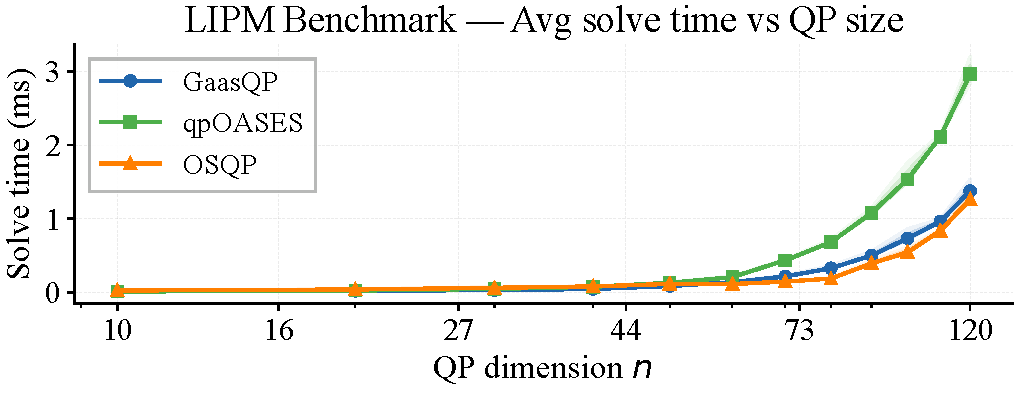
\includegraphics[width=0.95\linewidth]{figures_lipm/fig01_lipm_performance.pdf}
  \caption{Solve-time comparison on the LIPM walking MPC benchmark.
    Lines show the warm-run median over 30 repeats; shaded bands indicate
    the interquartile range and 5th--95th percentile.
    GeoQP exploits the block-diagonal Hessian structure via decoupled
    Schur complements and is consistently faster than qpOASES beyond $N=10$.
    OSQP under equal tolerance ($\varepsilon=10^{-7}$) is competitive at
    small horizons but slows substantially for $N\ge45$ due to the increasing
    spectral radius of the condensed LIPM Hessian.}
  \label{fig:lipm_timing}
\end{figure}

\begin{figure}[t]
  \centering
  \includegraphics[width=0.95\linewidth]{figures_lipm/fig03_violin.pdf}
  \caption{Algorithmic-effort distributions for GeoQP (Phase-3 pivot count)
    versus qpOASES (reported active-set iterations) at three representative
    horizons.
    GeoQP uses exactly $2$ pivots at all horizons owing to the decoupled
    x/y structure; facet-hop counts are identically $0$.
    qpOASES iteration counts grow with $N$ and exhibit larger variance.}
  \label{fig:lipm_hops}
\end{figure}